% Created 2021-01-24 Sun 22:50
% Intended LaTeX compiler: pdflatex
\documentclass[11pt]{article}
\usepackage[utf8]{inputenc}
\usepackage[T1]{fontenc}
\usepackage{graphicx}
\usepackage{grffile}
\usepackage{longtable}
\usepackage{wrapfig}
\usepackage{rotating}
\usepackage[normalem]{ulem}
\usepackage{amsmath}
\usepackage{textcomp}
\usepackage{amssymb}
\usepackage{capt-of}
\usepackage{hyperref}
\usepackage{minted}
\hypersetup{colorlinks=true, linkcolor=black, filecolor=red, urlcolor=blue}
\usepackage[turkish]{babel}
\author{Eren Hatırnaz}
\date{13 Ekim 2019}
\title{Yazılım Gündemi - 13\\\medskip
\large 7-13 Ekim 2019}
\hypersetup{
 pdfauthor={Eren Hatırnaz},
 pdftitle={Yazılım Gündemi - 13},
 pdfkeywords={},
 pdfsubject={},
 pdfcreator={Emacs 27.1 (Org mode 9.3)},
 pdflang={Turkish}}
\begin{document}

\maketitle
\tableofcontents \clearpage\shorthandoff{=}

\begin{center}
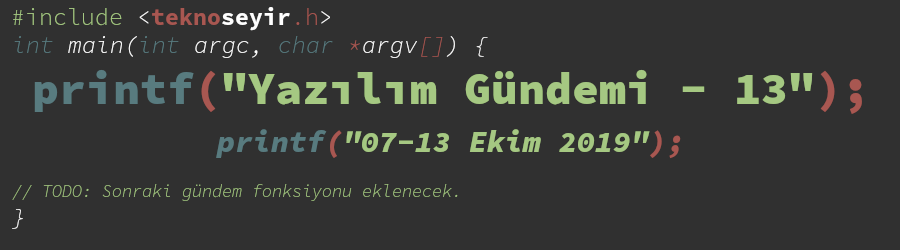
\includegraphics[width=.9\linewidth]{gorseller/yazilim-gundemi-banner.png}
\end{center}

\begin{center}
\href{../12/yazilim-gundemi-12.pdf}{< Önceki Gündem} | \textbf{7-13 Ekim 2019} | \href{../14/yazilim-gundemi-14.pdf}{Sonraki Gündem >}

\href{https://teknoseyir.com/blog/yazilim-gundemi-13-07-13-ekim-2019}{TeknoSeyir'de Oku}
\end{center}

\section{Github ile ABD Göçmenlik ve Gümrük Muhafaza kurumu arasındaki iş anlaşması \href{https://github.blog/2019-10-09-github-and-us-government-developers/}{tartışmalara yol açtı}}
\label{sec:orge845ac2}
Github ve ABD Göçmenlik ve Gümrük Muhafaza Kurumu arasındaki yaklaşık
200.000\$'lık bir iş anlamasının yenilenme zamanı gelince ortalık biraz karıştı.
Birkaç hafta önce de bir geliştiricinin aynı kurumu protesto etmek için yaptığı
bir eylemden bahsetmiştim (bkz: \href{../10/yazilim-gundemi-10.pdf}{Yazılım Gündemi - 10}). Amerika'da yaşamadığım
için doğal olarak bu kurum ve politikalarıyla ilgili bir bilgim yok fakat
insanların bu kadar fazla olay etmesine bakılırsa pek iyi bir kuruma
benzemiyor.

GitHub durumu açıklamak için tüm çalışanlarına gönderdiği e-postanın aynısını
bloglarında yayınladı. Olayın geçmişinden ve kendilerinin izledikleri rollerden
bahsetmişler. Kısaca özetlemek gerekirse: ilk iş anlaşması 2016 yılında
yapılıyor ve ilgili kurum GitHub Enterprise Server lisansı alıyor. Sanırım o
zamanlarda bu kurumun olay yaratan politikaları gündemde değilmiş. GitHub ve
Microsoft, ilgili kurumun olay yaratan politikalarına her ne kadar karşı
olsalar da "iş başka arkadaşlık başka" hesabıyla anlaşmaya devam ettiklerini
belirttiler. "Kurumun ilgili politikalarını her yerde protesto ettik ve etmeye
devam edeceğiz" deyip ekliyorlar: "Protesto amaçlı organizasyonlara
500.000\$'lık bağış yapacağız".

Twitter'daki \href{https://mobile.twitter.com/evan\_greer/status/1181745056698572802}{şu gönderi altında} bayağı bir tartışma dönmüş durumda. Bazı GitHub
ve Microsoft çalışanlarının da olayları \href{https://www.geekwire.com/2019/microsoft-github-workers-protest-ice-contracts-latest-demonstration-employee-activism/}{protesto ettiğine yönelik haberler var}.
Bakalım olaylar nereye varacak.
\section{GNU projesi geliştiricileri Richard M. Stallman'ın devam eden liderliğine \href{https://www.zdnet.com/article/gnu-project-developers-object-to-richard-m-stallmans-continued-leadership/}{itiraz ediyor}}
\label{sec:org9710863}
Geçtiğimiz haftalarda Richard M. Stallman'ın bazı söylemleri yüzünden Özgür
Yazılım Vakfı'ndaki (Free Software Foundation) ve MIT'deki görevinden
ayrıldığını konuşmuştuk (bkz: \href{../10/yazilim-gundemi-10.pdf}{Yazılım Gündemi - 10}). Sonraki haftalarda
Stallman, "FSF ve MIT'den istifa ettim fakat GNU projesine liderlik etmeye
devam ediyorum" şeklinde bir açıklama yaptı.

6 Ekim'de FSF \href{https://www.fsf.org/news/fsf-and-gnu}{şöyle bir yazı yayınladı} ve özgür yazılım topluluğundan durumla
ilgili görüşler toplamaya başladı. Bunun üzerine bazı GNU projesi
geliştiricileri de fikirleri açık şekilde bir yazı ile belirtmek için 7 Ekim'de
\href{https://guix.gnu.org/blog/2019/joint-statement-on-the-gnu-project/}{şu yazıyı yayınladılar}. Yazıca kısaca Richard Stallman'ın özgür yazılım
hareketinin ve GNU projesini ilk ortaya koyan ve büyük emekler veren kişi
olduğunu kabul ettiklerini fakat yıllar içerisinde Stallman'ın davranışlarının
değişmesinden dolayı artık GNU projesini temsil etmediğini düşündüklerini
belirtmişler.

10 Ekim tarihli bir güncelleme notu düşülen bu sayfada toplanan tüm görüşlerin
hem FSF hem de GNU liderliğiyle özel olarak paylaşıldığı belirtilmiş. Bakalım
süreç nasıl devam edecek. Sizin konu hakkındaki görüşleriniz nedir? Richard
Stallman tamamen yazılım camiasından dışlanmalı mıdır yoksa politik görüşleri
ayrı, programcı (hacker) kişiliği ayrı mı değerlendirilmelidir? Yorumlar
kısmında konuşalım.
\section{Chrome, geliştiricinin \texttt{autocomplete=off} \href{https://bugs.chromium.org/p/chromium/issues/detail?id=914451\#c73}{seçimine rağmen \texttt{autofill} özelliğini kapatmıyor}}
\label{sec:org6354061}
\texttt{Autocomplete} (otomatik tamamlama), kullanıcıların bir metin kutusuna
birşeyler yazarken daha önce yazdıklarını önermeye yarayan bir tarayıcı
özelliği. \texttt{autofill} (otomatik doldurma) ise sayfadaki bir formu, elemanların
\texttt{autocomplete} özelliğindeki değerlerden yararlanarak otomatik olarak
tarayıcıda kayıtlı değerlerle doldurmaya yarayan bir özellik. Örneğin bir
kullanıcı girişi formunda kullanıcı adınızı yazdıktan sonra şifre kutusunun da
otomatik olarak doldurulması. Çoğu durumda faydalı olabilirken bazen de
geliştirici için biraz sorunlu olabiliyor. Böyle durumların üstesinden gelmek
için de bu özelliği \texttt{input} bazında kapatmaya yarayan bir tercih
geliştiricilere sunulmuş fakat chrome'un buna tercihe saygı duymadığı,
\texttt{autocomplete=off} seçili olduğu halde otomatik doldurma özelliğini kapatmadığı
ortaya çıktı. Aslında bu yeni bir olay değil konu başlığına eklediğim
bağlantıdan da görebileceğiniz gibi ilgili issue 12 aralık 2018 tarihinde
açılmış fakat hala daha çözülmediği için tekrar gündeme geldi ve geliştiriciler
\href{https://www.reddit.com/r/programming/comments/dhd3av/issue\_914451\_autofill\_does\_not\_respect/}{sitemlerini belirtmeye devam ediyor}. Açıkcası Google'dan giderek daha da
soğuyan bir kişi olarak, bu durumdan da hiç haz etmedim. Resmen kodladığımız
siteye ve ona belirttiğimiz tercihlere aykırı hareket ediyor ve uzun zamandır
da hiçbir eylem alınmış değil. Google'a artık birilerinin dur demesi gerekiyor
ama kim ne zaman diyecek bilemiyoruz. Bakalım ne olacak. Siz bu konuda ne
düşünüyorsunuz?

\textbf{Düzeltme (14.10.2019 11:40)}: \texttt{autocomplete} ve \texttt{autofill} özelliklerinin
karıştırılmasından doğan yanlış anlaşılma sorunu giderildi.
\section{Visual Studio Code \href{https://code.visualstudio.com/updates/v1\_39}{Eylül 2019 (1.39) sürümü yayınlandı}}
\label{sec:orgeba1d8e}
\begin{center}
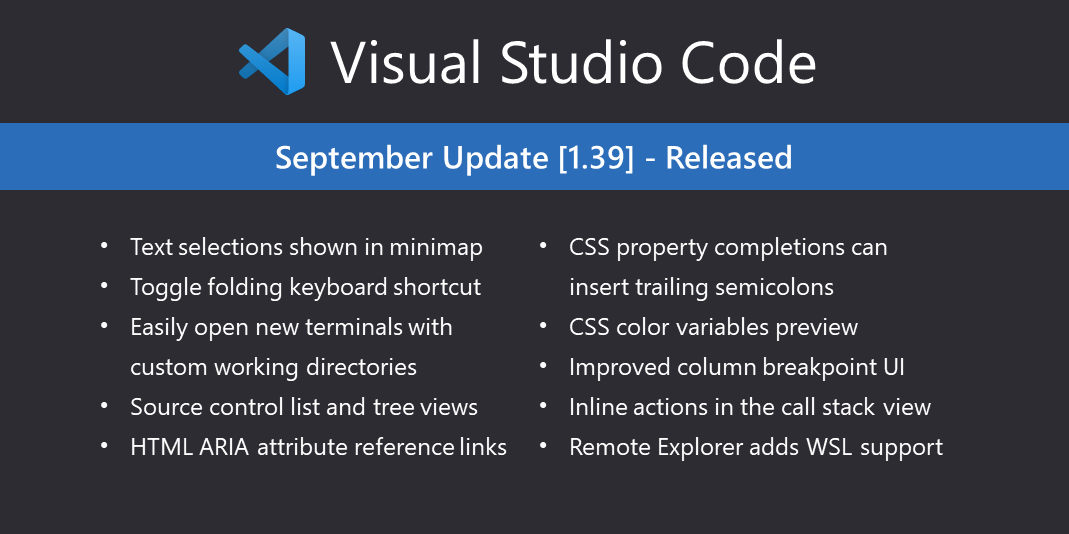
\includegraphics[width=.9\linewidth]{gorseller/vscode1-39.png}
\end{center}

Ayrıca Python eklentisinin bu ay duyurulan yeni sürümü ile VS Code'da artık
native olarak \href{https://devblogs.microsoft.com/python/announcing-support-for-native-editing-of-jupyter-notebooks-in-vs-code/}{Jupyter Notebook düzenleme özelliği de geldi}.
\newpage
\section{Yaklaşan Etkinlikler}
\label{sec:orga3714cf}
\begin{longtable}{|p{8cm}|l|l|}
\hline
Etkinlik İsmi & Yer & Tarihi\\
\hline
\endfirsthead
\multicolumn{3}{l}{Önceki sayfadan devam ediyor} \\
\hline

Etkinlik İsmi & Yer & Tarihi \\

\hline
\endhead
\hline\multicolumn{3}{r}{Devamı sonraki sayfada} \\
\endfoot
\endlastfoot
\hline
\href{https://kommunity.com/nsankara/events/ns-ankara-ekim-ayi-2-bulusma}{Managing Different Environments} & Ankara & 15 Ekim 18:30\\
\href{https://www.eventbrite.com/e/zebra-emea-android-developer-seminars-istanbul-2019-tickets-73787116251}{Zebra Emea Android Developer Seminars} & İstanbul & 16 Ekim 09:00\\
\href{https://www.eventbrite.com/e/trai-meet-up-27-yapay-zeka-altyaplar-tickets-73255123045}{TRAI Meet-Up \#27 Yapay Zekâ Altyapıları} & İstanbul & 16 Ekim 18:00\\
\href{https://www.eventbrite.com/e/yazlmda-kariyer19-tickets-75927901397}{Yazılımda Kariyer'19} & İstanbul & 16 Ekim 18:30\\
\href{https://kommunity.com/software-craftsmanship-turkey/events/kubernetes-operators-101}{Kubernetes Operators 101} & İstanbul & 16 Ekim 19:00\\
\href{https://www.eventbrite.com/e/kuantum-makine-ogrenmesi-tickets-76530519845}{Kuantum Makine Öğrenmesi} & İstanbul & 17 Ekim 18:30\\
\href{https://kommunity.com/devnot-yazilimci-bulusmalari/events/big-datadan-nasil-anlam-cikarabiliriz}{Big Data'dan Nasıl Anlam Çıkarılır?} & İstanbul & 18 Ekim 19:00\\
\href{https://kommunity.com/voistanbul/events/workshop-sesli-arayuzlerde-gorsel-cevaplar}{Workshop: Sesli Arayüzlerde Görsel Cevaplar} & İstanbul & 19 Ekim 11:00\\
\hline
\end{longtable}
\section{Diğer Haberler}
\label{sec:org3838a2b}
\begin{itemize}
\item Mozilla güvenlik takımı, \href{https://blog.mozilla.org/security/2019/10/09/iterm2-critical-issue-moss-audit/}{iTerm2'de kritik bir güvenlik açığı} buldu.
\item Yeni bir build ve test aracı: \href{https://bazel.build/}{Bazel}, \href{https://github.com/bazelbuild/bazel}{GitHub Deposu}.
\item Amazon Elastic Kubernetes Service içerisindeki \href{https://aws.amazon.com/tr/blogs/aws/amazon-eks-windows-container-support-now-generally-available/}{Windows Container desteği
artık herkese açık hale geldi}.
\item IoT için görsel programlama ortamı sunan \href{https://nodered.org/}{Node-RED} ilk \href{https://www.infoq.com/news/2019/10/nodered-1-0-released/}{stabil sürümü 1.0'ı
duyurdu}.
\item Mycroft isimli firma sesli asistan yazılımını AGPL lisansı ile \href{https://mycroft.ai/blog/open-sourcing-the-mycroft-backend/}{açık kaynak
hale getirdiler}. \href{https://github.com/MycroftAI}{Firmanın GitHub Sayfası}
\item Yeni bir LISP lehçesi duyuruldu: \href{https://sep.yimg.com/ty/cdn/paulgraham/bellanguage.txt?t=1570888282}{Bel}.
\item PyTorch \href{https://ai.facebook.com/blog/pytorch-13-adds-mobile-privacy-quantization-and-named-tensors/}{1.3 duyuruldu}.
\item OpenSSH \href{http://www.openssh.com/txt/release-8.1}{8.1 duyuruldu}.
\item JDK 14 sürümünde \href{https://openjdk.java.net/jeps/349}{JFR Event Streaming} özelliği \href{https://mail.openjdk.java.net/pipermail/jdk-dev/2019-October/003377.html}{gelecek}.
\item Next.js \href{https://github.com/zeit/next.js/releases/tag/v9.1.1}{9.1.1 sürümü yayınlandı}.
\item AndroidX WorkManager API \href{https://developer.android.com/jetpack/androidx/releases/work\#2.3.0-alpha02}{2.3.0-alpha02 sürümü çıktı}.
\item C kütüphanesi tbox, \href{https://tboox.org/2019/10/11/update-v1.6.4/}{1.6.4 sürümünü duyurdu}.
\end{itemize}
\section{Lisans}
\label{sec:orgaceec2e}
\begin{center}
\begin{center}

\includegraphics[height=1.5cm]{../../../img/CC_BY-NC-SA_4.0.png}
\end{center}

\href{yazilim-gundemi-13.pdf}{Yazılım Gündemi - 13} yazısı \href{https://erenhatirnaz.github.io}{Eren Hatırnaz} tarafından \href{http://creativecommons.org/licenses/by-nc-sa/4.0/}{Creative Commons
Atıf-GayriTicari-AynıLisanslaPaylaş 4.0 Uluslararası Lisansı} (CC BY-NC-SA 4.0)
ile lisanslanmıştır.
\end{center}
\end{document}
